\documentclass[sigconf,anonymous,review]{acmart}

\usepackage{amsmath}
\usepackage{booktabs}
\usepackage{graphicx}
\usepackage{multirow}
\usepackage{xcolor}
\usepackage{xspace}

\setcopyright{none}
\acmDOI{}
\acmISBN{}
\acmConference[WSDM '27]{The Twentieth ACM International Conference on Web Search and Data Mining}{February 15--19, 2027}{Hong Kong, China}
\acmYear{2027}
\copyrightyear{2027}

\newcommand{\system}{HCPM}

% AML internal review helpers; intentionally unused in the anonymous submission.
\newcommand{\zxy}[1]{{\color{blue} [#1 -- Xy]}}
\newcommand{\zc}{\textcolor{blue}{[cite]}\xspace}

\title{HCPM: Discovering Latent Habits for Controlled Proactive Memory in LLM Agents}

\author{Anonymous Author(s)}
\affiliation{\institution{Anonymous Institution}}

\begin{document}

\begin{abstract}
Long-term memory allows large language model agents to retain information beyond a single interaction, but retrieval alone does not determine when remembered information should interrupt an ongoing task.
This distinction is important for web-facing and tool-using agents: users may not fully articulate their recurring workflows, while an agent that surfaces every related memory becomes distracting.
We formulate proactive memory delivery as a turn-level decision problem and introduce \system{}, a middleware that discovers latent habits from interaction traces and controls whether they should be surfaced at the current turn.
\system{} consolidates repeated event--consequence patterns into typed habits, generalizes variable event forms, generates candidates from multiple trigger families, and applies scoring, phase-aware gating, and per-habit cooldown before producing a structured Push or no-Push decision.
Across six domain adaptations covering code, smart home, shopping, email, calendar, and project management, \system{} reaches a macro F1 of 0.653, compared with 0.392 for an oracle that selects the strongest evaluated proxy baseline independently in each domain.
It also reduces false positives from 604 to 176 and proactive pushes from 822 to 408 relative to those selected proxies.
Ablations show that generalized habit matching is the broadest contributor, while phase gating has a large, repeatable Code-specific effect.
Cooldown exposes a measurable recall--intervention trade-off rather than universally maximizing F1.
These results support a modular view of proactive memory: useful systems must discover unspoken regularities and separately control when acting on them is warranted.
\end{abstract}

\ccsdesc[500]{Information systems~Information retrieval}
\ccsdesc[300]{Computing methodologies~Artificial intelligence}
\ccsdesc[300]{Human-centered computing~Human computer interaction (HCI)}

\keywords{LLM agents, long-term memory, habit discovery, proactive assistance, intervention control}

\maketitle

\section{Introduction}
\label{sec:introduction}

Large language model (LLM) agents increasingly operate over web applications, workplace tools, software repositories, and personal services.
In these settings, an agent may interact with the same user and environment over many sessions.
Persistent-memory systems address this setting through complementary mechanisms, including storing and retrieving prior events, consolidating conversational facts, producing higher-level reflections, and organizing memories in hierarchical or graph-structured stores~\citep{park2023generative,packer2023memgpt,zhong2024memorybank,chhikara2025mem0,xu2025amem,gutierrez2024hipporag}.
These mechanisms answer an important question: \emph{what past information is relevant now?}
They do not, by themselves, answer a second question: \emph{should that information be surfaced at the current turn?}

The second question becomes central when memory is proactive.
A reactive system waits for a query; a proactive system may interrupt an ongoing workflow.
The cost of an incorrect decision is therefore asymmetric.
Missing a useful reminder loses an opportunity, while an unnecessary reminder consumes attention, may expose an incorrect inference about the user, and can steer an agent toward an action that was never intended.
Relevance is not enough: a memory can be related to the current task but premature, already satisfied, inconsistent with an explicit exception, or repeated too soon after an earlier intervention.

Recent preprints have begun to study streaming latent-need detection with hybrid memory, reasoning-integrated memory exploration, and selective reminder injection~\citep{xie2026pask,li2026memcog,wu2026remember}.
We focus on a complementary gap.
Users may not enumerate their own recurring workflows or express them as stable rules.
For example, a developer may regularly commit only after tests pass, a shopper may repeatedly avoid a class of ingredients, or a calendar user may follow a scheduling preference without ever declaring it as a memory.
An agent should be able to infer such regularities from interaction traces.
At the same time, the inferred habit must not become an unconditional notification rule.

We introduce \system{} (Habit-Consolidated Proactive Memory), a modular middleware for discovering latent habits and controlling their delivery.
\system{} observes structured user and agent events, accumulates repeated evidence, and consolidates trigger--context--consequence regularities into typed habit records.
It generalizes semantically equivalent event forms, generates proactive candidates through several trigger families, and exposes an auditable controller that scores candidates, checks workflow phase, optionally consults an LLM for high-risk cases, and enforces cooldown.
Its evaluated output is a structured Push or no-Push decision; optional natural-language realization occurs only after this decision and is outside the core mechanism.

This formulation is relevant to web search and data mining in two ways.
First, web agents and intelligent assistants must mine longitudinal interaction traces rather than treat each request independently.
Second, the utility of retrieved behavioral evidence depends on decision timing: the system must rank candidate memories and decide whether any candidate should enter the current agent context.
The resulting problem joins behavioral pattern mining, retrieval, and selective intervention for agentic systems.

We make four contributions:
\begin{itemize}
    \item We formulate proactive memory as a turn-level decision problem and construct six controlled domain adaptations grounded in public commit histories and public WorkBench, $\tau$-bench Retail, and SmartBench sources. These are adaptations, not official-protocol benchmark scores.
    \item We present \system{}, which discovers habits that need not be explicitly declared and couples generalized habit matching with an auditable intervention controller.
    \item We provide six-domain effectiveness, ablation, statistical, repeatability, and error evidence. \system{} improves macro F1 from 0.392 for the strongest evaluated per-domain proxy baselines to 0.653, while its mechanisms activate under different domain structures.
    \item We test targeted mechanism effects across four model configurations and report absolute call and token composition without claiming matched-baseline efficiency superiority.
\end{itemize}

\section{Problem Formulation}
\label{sec:problem}

\subsection{Events, Habits, and Decisions}

Let a session be an ordered stream of events $E=(e_1,\ldots,e_T)$.
Each event is represented as
\begin{equation}
e_t=(\tau_t,a_t,v_t,o_t,m_t)
\end{equation}
Here, $\tau_t$ is time, $a_t$ is the actor, $v_t$ is an action verb, $o_t$ is an object or entity, and $m_t$ contains domain metadata.
Structured tool calls are mapped deterministically; free-form language can be parsed into the same schema by an LLM.
The benchmark uses pre-structured events so event parsing is not part of the reported decision accuracy.

A habit $h$ represents a recurring behavioral regularity:
\begin{equation}
h=(g_h,c_h,k_h,q_h,f_h,\rho_h,z_h,V_h)
\end{equation}
Here, $g_h$ is a trigger action--entity pattern, $c_h$ is trigger context, $k_h$ records consequence statistics over observed typical outcomes, $q_h$ is confidence, $f_h$ and $\rho_h$ encode frequency and recency, $z_h$ is lifecycle state, and $V_h$ is a set of generalized variants.
Habit types include workflow, temporal, emotional, and associative patterns.

At each turn, the system observes the current event and memory state $M_t$, and outputs
\begin{equation}
\hat{y}_t = \pi(e_{\leq t},M_t) \in \{0,1\}
\end{equation}
Here, $1$ denotes a structured Push decision.
When $\hat{y}_t=1$, the decision also identifies its trigger, supporting habit, candidate score, and control trace.
Natural-language wording is a downstream host-system concern and does not change $\hat{y}_t$.

\subsection{Evaluation Objective}

Each evaluation turn has a ground-truth label $y_t$ indicating whether an intervention is useful at that stage.
We report precision, recall, F1, false positives (FP), and Push count in the main text; complete traces additionally retain accuracy and true-positive, false-negative, and true-negative counts.
F1 captures the balance between recovering useful interventions and avoiding false ones, while FP and Push count directly report false and total intervention frequency; they are offline proxies for potential intervention burden rather than measurements of perceived burden, satisfaction, trust, or helpfulness.
No single metric fully represents user utility: the relative cost of one missed intervention and one unnecessary interruption is deployment dependent.
We therefore treat threshold and cooldown as an operating policy rather than tune them solely to maximize test F1.

\section{HCPM Framework}
\label{sec:framework}

\subsection{Overview}

Figure~\ref{fig:architecture} summarizes the pipeline.
\system{} separates two responsibilities.
The \emph{discovery layer} turns repeated interaction evidence into typed, persistent habits.
The \emph{control layer} decides whether a habit-derived candidate is actionable at the current turn.
This separation prevents ``memory found'' from becoming synonymous with ``notification sent.''

\begin{figure*}[t]
    \centering
    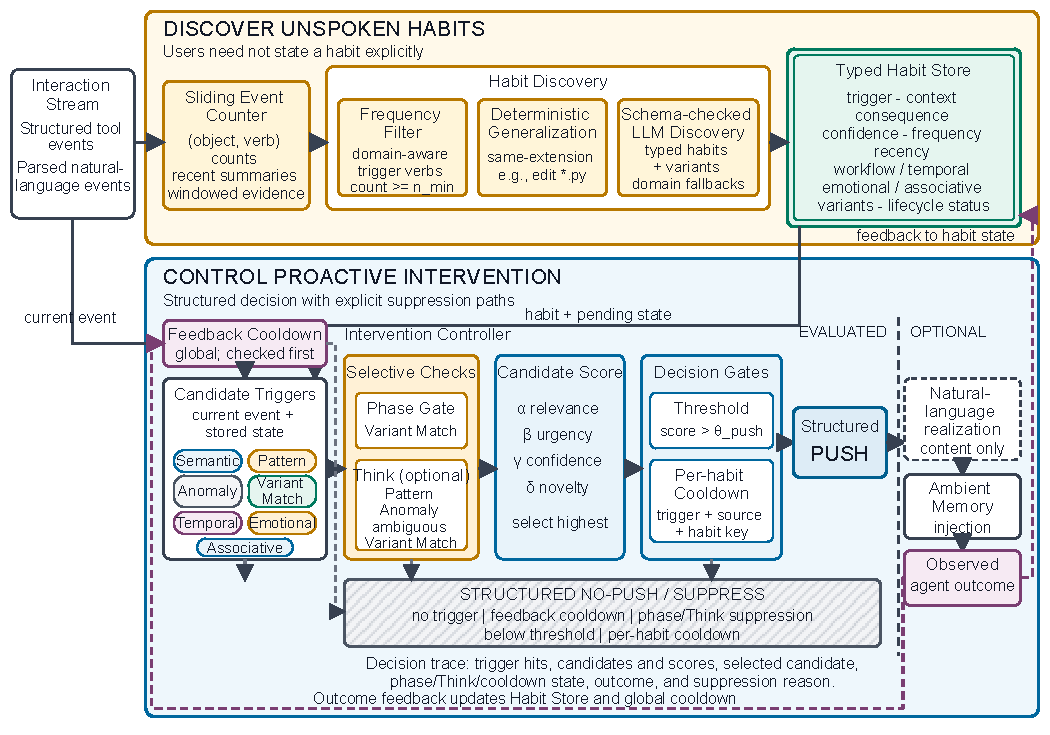
\includegraphics[width=\textwidth,page=1]{sampleteaser.pdf}
    \Description{A two-band HCPM architecture diagram. The upper band discovers typed habits from interaction events; the lower band generates, scores, suppresses, or delivers proactive candidates. A dashed boundary separates the evaluated Push/no-Push decision from optional language realization, and a feedback arrow returns observed outcomes to habit and cooldown state.}
    \caption{\system{} architecture and evaluated decision boundary. The framework separates discovery of recurring, unspoken habits from control of proactive intervention. Seven trigger families produce candidates; selective phase/Think checks, weighted scoring, a threshold, and cooldowns yield a structured Push/no-Push decision. Optional natural-language realization lies outside the evaluated decision boundary, while observed use or non-use feeds back to habit and cooldown state.}
    \label{fig:architecture}
\end{figure*}

\subsection{Event Accumulation and Habit Discovery}

An event counter maintains frequencies of $(o,v)$ pairs and a sliding buffer of recent event summaries.
Every discovery batch filters out conversational, terminal, and verification actions that should not independently define a habit.
Candidates must have at least $n_{\min}=3$ supporting events in the default configuration.
For coding events, deterministic preprocessing merges repeated files with the same extension (e.g., several Python edits can become \texttt{edit *.py}); domains with normalized entities retain their verb--object keys.

The remaining evidence is passed to an LLM with a constrained schema.
The output proposes a habit type, trigger, trigger context, consequence, and variants.
The parser removes reasoning blocks, scans for a schema-valid JSON payload, and retries malformed outputs before applying domain-specific fallbacks.
Thus, the LLM proposes structured regularities, while deterministic checks govern admissible evidence and the representation written to memory.
Users need not state ``this is my habit,'' but the system still requires repeated observational evidence and does not claim zero-history personalization.

\subsection{Habit Confidence and Lifecycle}

Each record tracks frequency, last observation, consequence statistics, confidence, and lifecycle state.
Let
\begin{align}
F(h) &= \min(f_h/f_{\max},1)\\
R(h) &= \exp(-\lambda \Delta_h)
\end{align}
Here, $\Delta_h$ is days since the last observation.
We use $f_{\max}=20$. The consistency term is $C(h)=1.0$ for at most two distinct consequences, $0.7$ for three to four, and $0.4$ for five or more.
The implementation computes
\begin{equation}
q_h=\sigma\!\left(6\left[w_fF(h)+w_rR(h)+w_cC(h)-0.5\right]\right)
\end{equation}
Here, $\sigma$ is the logistic sigmoid, $(w_f,w_r,w_c)=(0.5,0.3,0.2)$, and $\lambda=0.1$.
Records transition among active, fading, forgotten, and abandoned states; repeated evidence can reinforce a fading record.
The current implementation persists the Habit Store; counters and queues are maintained as runtime state and could in principle be rebuilt by replaying the event stream.

\subsection{Generalized Habit Matching}

Exact matching is brittle when behavior is stable but surface forms vary.
\system{} therefore stores generalized trigger patterns and variants.
A coding habit may match a glob pattern, while preference-oriented domains can map an observed conflict key to a normalized habit entity.
At runtime, Variant Match selects the highest-confidence supported variant and emits a candidate describing the typical consequence.
The Exact-only ablation retains habit discovery but disables generalized runtime matching, isolating the value of abstraction beyond literal event equality.

\subsection{Multi-Source Candidate Generation}

The controller supports seven trigger families:
\begin{itemize}
    \item \textbf{Semantic}: queries an optional external vector store with \texttt{top\_k=3} and emits a candidate from the best returned item only when its score strictly exceeds $0.75$.
    \item \textbf{Pattern}: fires when an expected consequence remains unfulfilled past its time window.
    \item \textbf{Anomaly}: detects a structurally related action that deviates from a high-confidence habit.
    \item \textbf{Variant Match}: matches the current action to a discovered exact or generalized habit variant.
    \item \textbf{Temporal}: activates a typed temporal habit at a compatible time.
    \item \textbf{Emotional}: matches stored emotional cues or keywords.
    \item \textbf{Associative}: surfaces a habit through an associated concept.
\end{itemize}

Each candidate $c$ has relevance $r_c$, urgency $u_c$, confidence $q_c$, and novelty $n_c$.
The score is
\begin{equation}
s(c)=0.35r_c+0.25u_c+0.25q_c+0.15n_c
\end{equation}
The highest-scoring candidate proceeds only if $s(c)>\theta_{\mathrm{push}}$, with $\theta_{\mathrm{push}}=0.6$ by default.

\subsection{Phase-Aware and Confidence-Aware Control}

Related behavior is not necessarily actionable behavior.
For workflow domains with observable execution stages, \system{} derives a compact phase from recent events.
In Code, for example, current test status and edit/run/debug activity distinguish early work, implementation, debugging, documentation work, and wrap-up.
A matching habit can be suppressed during early work or active debugging and allowed after stable verification.
For non-coding domains where those signals do not apply, the phase module returns an active state rather than imposing coding-specific rules.

Pattern and Anomaly candidates may pass through the optional LLM Think check when Think is enabled and an LLM is available.
In the Code workflow path, a Variant Match candidate may also invoke Think when the detected phase is early or implementing; with Think disabled or no LLM available, that branch applies deterministic phase suppression.
For Variant Match, debugging is suppressed directly by the phase gate; candidates admitted in any other phase remain subject to the score threshold and cooldown rather than being pushed unconditionally.
The checker receives current phase, recent actions, test state, and the candidate, then returns PUSH or SUPPRESS with a confidence value.
An LLM-call failure is recorded and returns the candidate to the structured decision path, which still applies downstream candidate selection, thresholding, and cooldown.
As Section~\ref{sec:ablation} shows, this checker has only weak and unstable marginal evidence in the current experiments; it is retained as an optional safeguard rather than presented as the central contribution.

\subsection{Cooldown and Feedback Control}

After thresholding, a candidate is checked against a cooldown key formed from trigger and source, with the habit identifier appended when available.
Habit-backed candidates can therefore maintain independent cooldowns, while candidates without a habit identifier use the trigger--source key as a fallback.
The frozen experiments use a three-event cooldown, reset at session boundaries.
After an observed response to a Push, a global feedback cooldown can also suppress immediate follow-up notifications, whether the suggestion was used or ignored.

Cooldown determines an intervention operating point.
It is not a categorical user-interface label and is not expected to maximize F1 in every domain.
The complete decision trace stores the candidate, phase, Think result, cooldown distance, suppression reason, and final outcome, allowing an evaluator to distinguish absent evidence from deliberate suppression.

\subsection{Deployment Boundary}

The structured decision is middleware output.
An agent host may inject it directly, transform it into a notification, request confirmation, or suppress it under an application policy.
Optional LLM rewriting occurs after selection and cooldown and therefore does not alter decision F1.
We report this cost separately in Section~\ref{sec:efficiency}.

\section{Experimental Setup}
\label{sec:setup}

\subsection{Research Questions}

We study four questions: (RQ1) Does \system{} improve proactive decision quality over the evaluated memory proxies? (RQ2) Which mechanisms contribute under different domain structures? (RQ3) Are the effects stable across repetitions, protocols, and model configurations? (RQ4) What is the measured call and token composition of the framework?

\subsection{Domains and Data Construction}

Table~\ref{tab:data} summarizes the evaluation data.
Code is a real-world-grounded controlled adaptation rather than a direct replay of raw developer logs.
We mined public commit histories from five open-source repositories---Requests, Flask, HTTPX, tqdm, and FastAPI---and used representative bug-fix, feature, documentation, configuration, and refactoring activities to inform the scenario design.
We then expanded these activities into multi-turn repository workflows with explicit edit, test, debug, and commit stages.
Code Push labels follow pre-specified observable workflow rules that are independent of \system{}'s predictions and internal phase detector.
Email, Calendar, and Project Management are HCPM adaptations of records and task structures from WorkBench~\citep{styles2024workbench}; Shopping is an HCPM adaptation of the Retail domain in $\tau$-bench~\citep{yao2025taubench}; SmartHome is an HCPM adaptation of the public SmartBench repository (accessed July 14, 2026; local snapshot commit \texttt{98bec394})~\citep{horizonsinzqs2026smartbench}.
We transform these sources into longitudinal event sessions and assign turn-level intervention labels using domain-specific construction rules.
The evaluated sessions contain 51 positive turns in Code, 42 in SmartHome, and 52 in each of the other four domains.
These controlled labels make intervention timing reproducible but are not annotations of naturally occurring longitudinal agent--user interactions.
The reported numbers are not directly comparable to official, unmodified benchmark leaderboards.

\begin{table}[t]
\centering
\caption{Dataset statistics. C/H denote clean/hard subsets. Warm-up events are excluded from evaluated turns.}
\label{tab:data}
\small
\begin{tabular}{lrrrr}
\toprule
Domain & C sess. & H sess. & Turns & Warm-up \\
\midrule
Code & 20 & 12 & 448 & 34 \\
SmartHome & 20 & 12 & 440 & 50 \\
Shopping & 20 & 12 & 495 & 54 \\
Email & 25 & 12 & 684 & 54 \\
Calendar & 25 & 12 & 684 & 54 \\
Project Mgmt. & 25 & 12 & 684 & 54 \\
\bottomrule
\end{tabular}
\end{table}

Clean sessions contain clearer evidence and expected intervention stages.
Hard sessions add premature cues, implicit positives, aligned actions, and explicit exceptions.
The main \texttt{all} condition is a continual stateful clean-to-hard run: the Habit Store, counter state, and learned variants persist across the subset boundary, while session-local cooldown is reset.
We separately audited split-reset and reversed-order protocols rather than treating \texttt{all} as a simple arithmetic union.

\subsection{Baselines}

All methods receive the same domain data and current event, use the same ground-truth labels, and produce the same Push/no-Push output under protocol-aligned evaluators; \system{} and the baseline families are executed by separate implementations rather than a shared internal execution path.
\textbf{No Memory} uses only the current event and short local context.
\textbf{Retrieval-augmented generation (RAG)-only} stores raw historical events and retrieves similar observations.
\textbf{Summary-Reflection} compresses observations into a long-term natural-language summary and reflections.
\textbf{Generative Memory} follows a relevance--recency--importance retrieval scheme inspired by Generative Agents~\citep{park2023generative}.
These baselines are local proxy implementations constructed for this study, not official reproductions of the named systems.
Across all baseline agents, the decision prompt includes at most 10 recent events in addition to the current event.
RAG-only ranks raw events by Jaccard token overlap; RAG-only and Generative Memory cap retrieval at \texttt{top\_k}=8.
Summary-Reflection updates every 20 observations, flushes any nonempty remainder at the end of warm-up, and retains at most 12 reflections.
Generative Memory uses Jaccard overlap as relevance and scores observations as $0.55\,\mathrm{relevance}+0.25\exp(-\mathrm{age}/80)+0.20\,\mathrm{importance}$, where age is observation-index distance.
Importance starts at 0.45, adds 0.25 for predefined action verbs, 0.20 for predefined salient terms, and 0.10 for user-authored events, and is capped at 1.0.
The baselines intentionally exclude \system{}'s typed Habit Store, generalized preference abstraction, and consolidation mechanism.
Warm-up and a per-memory cooldown of three events are applied where supported to avoid giving \system{} an intervention-frequency advantage by protocol alone.

\subsection{Metrics and Statistical Tests}

We compute precision, recall, F1, accuracy, true positives (TP), false positives (FP), false negatives (FN), true negatives (TN), and Push count from complete decision traces, while the main table presents precision, recall, F1, FP, and Push count.
For ablations, 95\% confidence intervals (CIs) use 10,000 paired, stratified session-level bootstrap samples, preserving within-session dependence and clean/hard stratum sizes, with fixed seed \texttt{20260713}.
Because turns within a session are dependent, inferential claims rely on these paired session-level intervals rather than treating individual turns as independent observations.
For Code and Calendar, the bootstrap analyses use validated Full repeat-2 traces as references because the original Full logs predate structured tracing; the reference traces reproduce the frozen Full predictions and confusion matrices.

\subsection{Implementation and Reproducibility}

The main matrix uses DeepSeek-V4-Flash with temperature zero, domain-specific warm-up, LLM Think enabled, and cooldown three.
The package requires Python 3.10 or newer; the current bundled audit runtime reports Python 3.12.13, while exact historical environments are not recoverable for every run.
Package defaults are a 30-event discovery window, a 30-minute consequence window, high-confidence and forgetting thresholds of 0.8 and 0.2, a 10-event candidate cooldown, and a five-event feedback cooldown. The frozen evaluators use a 50-event discovery window and override the candidate cooldown to three events.
The instrumented HCPM ablation, repeatability, cross-model, and efficiency evaluators write one JSON Lines (JSONL) decision trace per evaluated turn, containing trigger hits, candidates, score components, phase, Think output, cooldown state, ground truth, and TP/FP/FN/TN classification.
The source-level audit validates 90/90 main-result artifacts (72 baseline JSON result files and 18 HCPM source logs), while the manifest separately validates 36,779/36,779 JSONL rows across 65 instrumented HCPM runs.
Application programming interface (API) keys and endpoint credentials are excluded from the artifact.
None of the six frozen benchmark evaluators supplies \texttt{query\_vector\_store}; consequently, the external-vector Semantic branch is inactive in all reported experiments.
The gains observed in the four domains with semantic surface variation---Shopping, Calendar, Email, and Project Management---come from generalized Habit Variant Match rather than Semantic vector retrieval.

\section{Results and Analysis}
\label{sec:results}

\subsection{Overall Performance}

Table~\ref{tab:main_results} reports the continual \texttt{all} protocol results.
\system{} has the highest F1 in all six domains.
Its macro F1 is 0.653, compared with 0.388 for RAG-only and 0.392 for an oracle that chooses the strongest evaluated proxy baseline separately in each domain.

% Auto-generated from formal_results.csv by paper/assets/asset_build.py.
% Requires: booktabs, multirow, ulem (or soul) for underline.
\begin{table*}[t]
\centering
\caption{Six-domain continual stateful (\texttt{all}) results with DeepSeek-V4-Flash and cooldown 3. The datasets include task-specific adaptations and these values must not be interpreted as official benchmark scores. Best domain F1 is bold; second-best is underlined.}
\label{tab:main_results}
\footnotesize
\setlength{\tabcolsep}{5.0pt}
\begin{tabular}{llrrrrr}
\toprule
Domain & Method & P & R & F1 & FP & Pushes \\
\midrule
\multirow{5}{*}{Code} & No Memory & 0.000 & 0.000 & 0.000 & 1 & 1 \\
 & RAG-only & 0.161 & 0.529 & \underline{0.247} & 141 & 168 \\
 & Summary-Reflection & 0.120 & 0.333 & 0.176 & 125 & 142 \\
 & Generative Memory & 0.132 & 0.392 & 0.197 & 132 & 152 \\
 & HCPM & 0.617 & 0.725 & \textbf{0.667} & 23 & 60 \\
\addlinespace[1.5pt]
\multirow{5}{*}{SmartHome} & No Memory & 0.500 & 0.048 & 0.087 & 2 & 4 \\
 & RAG-only & 0.248 & 0.810 & \underline{0.380} & 103 & 137 \\
 & Summary-Reflection & 0.203 & 0.690 & 0.314 & 114 & 143 \\
 & Generative Memory & 0.238 & 0.738 & 0.360 & 99 & 130 \\
 & HCPM & 0.550 & 0.786 & \textbf{0.647} & 27 & 60 \\
\addlinespace[1.5pt]
\multirow{5}{*}{Shopping} & No Memory & 0.281 & 0.481 & 0.355 & 64 & 89 \\
 & RAG-only & 0.281 & 1.000 & \underline{0.439} & 133 & 185 \\
 & Summary-Reflection & 0.283 & 0.500 & 0.361 & 66 & 92 \\
 & Generative Memory & 0.273 & 0.981 & 0.427 & 136 & 187 \\
 & HCPM & 0.569 & 0.635 & \textbf{0.600} & 25 & 58 \\
\addlinespace[1.5pt]
\multirow{5}{*}{Email} & No Memory & 0.533 & 0.154 & 0.239 & 7 & 15 \\
 & RAG-only & 0.349 & 0.846 & \underline{0.494} & 82 & 126 \\
 & Summary-Reflection & 0.357 & 0.385 & 0.370 & 36 & 56 \\
 & Generative Memory & 0.262 & 0.731 & 0.386 & 107 & 145 \\
 & HCPM & 0.581 & 0.827 & \textbf{0.683} & 31 & 74 \\
\addlinespace[1.5pt]
\multirow{5}{*}{Calendar} & No Memory & 0.326 & 0.269 & 0.295 & 29 & 43 \\
 & RAG-only & 0.247 & 0.827 & 0.381 & 131 & 174 \\
 & Summary-Reflection & 0.435 & 0.385 & \underline{0.408} & 26 & 46 \\
 & Generative Memory & 0.253 & 0.885 & 0.393 & 136 & 182 \\
 & HCPM & 0.566 & 0.827 & \textbf{0.672} & 33 & 76 \\
\addlinespace[1.5pt]
\multirow{5}{*}{Project Management} & No Memory & 0.167 & 0.019 & 0.034 & 5 & 6 \\
 & RAG-only & 0.256 & 0.788 & \underline{0.387} & 119 & 160 \\
 & Summary-Reflection & 0.267 & 0.385 & 0.315 & 55 & 75 \\
 & Generative Memory & 0.214 & 0.769 & 0.335 & 147 & 187 \\
 & HCPM & 0.537 & 0.827 & \textbf{0.652} & 37 & 80 \\
\midrule
\multicolumn{7}{l}{\footnotesize Macro F1: No Memory 0.168; RAG-only 0.388; Summary-Reflection 0.324; Generative Memory 0.350; HCPM 0.653} \\
\bottomrule
\end{tabular}
\end{table*}

Compared with the strongest evaluated proxy baseline in each domain, the F1 gains are 0.420 (Code), 0.267 (SmartHome), 0.161 (Shopping), 0.188 (Email), 0.264 (Calendar), and 0.265 (Project Management).
The selected baselines produce 604 false positives and 822 pushes, whereas \system{} produces 176 false positives and 408 pushes, reductions of 70.9\% and 50.4\%, respectively.

The aggregate does not imply uniform metric dominance.
In Shopping, recall-heavy RAG-only reaches 1.000 recall but produces 133 false positives; \system{} reaches 0.635 recall with 25 false positives.
In Calendar, \system{} improves F1 and recall but produces 33 false positives, seven more than the best-F1 Summary-Reflection baseline.
These cases motivate reporting intervention count alongside F1.

\subsection{Mechanism Ablations}
\label{sec:ablation}

Table~\ref{tab:ablations} shows a modular rather than universally additive system; Full denotes the complete \system{} configuration under the frozen protocol.
Exact-only retains discovered habits but removes generalized runtime matching.
Removing the phase gate changes Code substantially but is prediction-identical in four other tested domains.

% Auto-generated from final_ablation_table.csv by paper/assets/asset_build.py.
% Requires: booktabs.
\begin{table*}[t]
\centering
\caption{Mechanism ablations. Cells report F1 (change from Full); an em dash denotes an untested setting. Generalized matching is active in Shopping, Calendar, Email, and Project Management; Phase Gate has a repeatable Code effect; the marginal Think effect is weak/unstable; cooldown selects an intervention operating point rather than universally improving F1.}
\label{tab:ablations}
\footnotesize
\setlength{\tabcolsep}{3.4pt}
\begin{tabular}{lccccc}
\toprule
Domain & Full & Exact-only & w/o Phase Gate & w/o LLM Think & w/o Cooldown \\
\midrule
Code & 0.667 (ref.) & 0.667 (+0.000) & 0.462 (-0.205) & 0.642 (-0.024) & \textemdash \\
SmartHome & 0.647 (ref.) & 0.647 (+0.000) & 0.647 (+0.000) & \textemdash & \textemdash \\
Shopping & 0.600 (ref.) & 0.429 (-0.171) & 0.600 (+0.000) & 0.600 (+0.000) & 0.701 (+0.101) \\
Email & 0.683 (ref.) & 0.197 (-0.486) & 0.683 (+0.000) & \textemdash & \textemdash \\
Calendar & 0.672 (ref.) & 0.133 (-0.539) & \textemdash & \textemdash & \textemdash \\
Project Management & 0.652 (ref.) & 0.143 (-0.509) & 0.652 (+0.000) & \textemdash & \textemdash \\
\bottomrule
\end{tabular}
\end{table*}

\textbf{Generalized matching.}
Full exceeds Exact-only in Shopping, Calendar, Email, and Project Management, with session-bootstrap intervals excluding zero: $[0.061,0.298]$, $[0.351,0.700]$, $[0.292,0.668]$, and $[0.311,0.677]$, respectively.
Code and SmartHome are exact negative controls with identical predictions.
Thus abstraction is most useful when preferences or workflow entities vary semantically, not when normalized events already match literally.

\textbf{Phase gate.}
Removing the gate lowers Code F1 by 0.205 (95\% CI $[0.131,0.276]$) and increases FP from 23 to 59.
The effect is repeatable across three runs, while four non-Code domains are prediction-identical with and without the gate.

\textbf{Think.}
Code w/o Think has a three-run mean F1 of 0.659 versus 0.667 for Full, and two repeats are prediction-identical to Full.
We therefore do not claim a robust aggregate contribution from the optional LLM checker.

\textbf{Cooldown.}
Removing Shopping cooldown raises turn-level F1 from 0.600 to 0.701 by increasing recall, but pushes rise from 58 to 85 and false positives from 25 to 37.
At cooldown three, 27 candidates are suppressed: 15 potential true positives and 12 potential false positives.
Cooldown therefore encodes an intervention-cost policy rather than an accuracy-only improvement.

Figure~\ref{fig:cooldown} makes the corresponding operating-point trade-off explicit.
\begin{figure}[t]
    \centering
    \includegraphics[width=\columnwidth,page=2]{sampleteaser.pdf}
    \Description{A single-column plot of tested Shopping cooldown settings. Cooldowns zero through two share one operating point; cooldown three lowers pushes and false positives while also reducing recall and F1. An inset decomposes 27 suppressed candidates into 15 potential true positives and 12 potential false positives.}
    \caption{Shopping cooldown operating points. Cooldown 0--2 and cooldown 3 are the discrete tested points; the connector is only a visual guide. Cooldown 3 suppresses both potential true and false interventions, illustrating an intervention-cost operating point rather than a setting that universally improves F1.}
    \label{fig:cooldown}
\end{figure}

\subsection{Stability Across Models and Protocols}

We repeat targeted Full--ablation comparisons with DeepSeek-V4-Pro, a gateway-reported GPT-5.5 endpoint, and MiniMax-M3.
Table~\ref{tab:cross_model} reports $\Delta\mathrm{F1}=\mathrm{Full}-\mathrm{Ablation}$.
All six selected effects replicate, including SmartHome as a zero-effect control.
Exact score equality across several configurations reflects identical decision traces under the tested structured protocol; it should not be interpreted as independent verification of endpoint identity.

% Auto-generated from four_model_comparison.csv by paper/assets/asset_build.py.
% Requires: booktabs.
\begin{table*}[t]
\centering
\caption{Cross-model replication of the selected mechanism effect. Effect is Full F1 minus ablated F1, so positive values indicate the same degradation after ablation. SmartHome Exact-only is a zero-effect control.}
\label{tab:cross_model}
\footnotesize
\setlength{\tabcolsep}{4.4pt}
\begin{tabular}{llrrrrc}
\toprule
Domain & Ablation & Flash & Pro & GPT-5.5 & MiniMax-M3 & Effect replicated \\
\midrule
Code & w/o Phase Gate & +0.205 & +0.184 & +0.184 & +0.184 & Yes \\
SmartHome & Exact-only & +0.000 & +0.000 & +0.000 & +0.000 & Yes \\
Shopping & Exact-only & +0.171 & +0.171 & +0.171 & +0.171 & Yes \\
Email & Exact-only & +0.486 & +0.486 & +0.486 & +0.486 & Yes \\
Calendar & Exact-only & +0.539 & +0.539 & +0.539 & +0.539 & Yes \\
Project Management & Exact-only & +0.509 & +0.509 & +0.509 & +0.509 & Yes \\
\bottomrule
\end{tabular}
\vspace{2pt}
\parbox{0.98\textwidth}{\footnotesize The GPT-5.5 model identity is gateway-reported and was not independently verified. The table supports replication of the selected effect, including the zero-effect control, not universal component effectiveness.}
\end{table*}

Code Full and Calendar Full each produce identical F1 in three observed repeats.
The Shopping protocol audit additionally compares continual, split-reset, and reversed orderings; these checks preserve the principal conclusion while clarifying that the main \texttt{all} run is stateful and must not be reconstructed by summing standalone splits.

\subsection{Efficiency Composition}
\label{sec:efficiency}

Table~\ref{tab:efficiency} reports absolute \system{} telemetry.
Across six Full runs, the framework makes 496 logical calls and observes 732,409 provider-reported tokens.
Discovery and Think account for 88 calls; optional Push formatting accounts for 408 calls (82.3\%) and 272,043 tokens (37.1\%).
Because formatting follows the structured decision, a host can replace it without changing F1.

\begin{table}[t]
\centering
\caption{Absolute Full-run telemetry under MiniMax-M3. Tokens are provider-reported observations.}
\label{tab:efficiency}
\small
\begin{tabular}{lrrr}
\toprule
Domain & Turns & Calls & Tokens \\
\midrule
Code & 448 & 105 & 112,287 \\
Shopping & 495 & 70 & 164,066 \\
Calendar & 684 & 85 & 125,510 \\
Email & 684 & 83 & 119,712 \\
Project Mgmt. & 684 & 89 & 123,218 \\
SmartHome & 440 & 64 & 87,616 \\
\midrule
Total & 3,435 & 496 & 732,409 \\
\bottomrule
\end{tabular}
\end{table}

Two optional Calendar formatting calls fail without usage payloads, so the token total is a lower bound.
Three serial Code measurements have an identical 105-call decomposition and identical decisions; the mean observed token count is 116,758 (sample standard deviation 4,514).
We do not compare these values with matched-model baseline telemetry and therefore make no baseline-relative efficiency claim.

\subsection{Error Analysis}

Errors concentrate at the boundary between retrieving a related habit and deciding that it is actionable.
In Code-hard, 11/17 false positives occur in aligned or exception negatives, while other errors push on early edits and miss the valid wrap-up stage.
Shopping-hard similarly contains premature pushes before final decision points and false positives on preference-aligned actions.
In Calendar-all, at least 20/33 false positives are directly verified as aligned or exception cases.

These errors identify three remaining weaknesses.
First, stage cues outside Code are less explicit, so relevant habits can fire before an actionable decision.
Second, a related preference is sometimes mistaken for a violated preference.
Third, implicit semantic evidence is weaker than explicit normalized conflict keys.
The findings support the architectural separation in Figure~\ref{fig:architecture}: habit discovery can succeed while push control still fails.

\section{Related Work}
\label{sec:related}

\subsection{Long-Term Memory for LLM Agents}

Generative Agents store observations, retrieve memories by relevance, recency, and importance, and synthesize higher-level reflections~\citep{park2023generative}.
Reflexion maintains reflective textual feedback in episodic memory across trials~\citep{shinn2023reflexion}, while MemoryBank maintains persistent conversational memories and updates their strength as interactions evolve over time~\citep{zhong2024memorybank}.
MemGPT treats limited context as a hierarchy of memory tiers~\citep{packer2023memgpt}.
Mem0 dynamically extracts, consolidates, and retrieves conversational memories and includes a graph-based variant~\citep{chhikara2025mem0}, whereas A-Mem organizes memory notes through dynamically generated links and updates existing representations as new memories arrive~\citep{xu2025amem}.
HippoRAG uses graph structure and personalized PageRank for cross-passage integration~\citep{gutierrez2024hipporag}.
These works motivate persistent and structured memory, but their principal evaluation target is storage, retrieval, response quality, or memory organization rather than turn-level intervention timing.

\subsection{Memory Evaluation}

LoCoMo evaluates long-term conversational memory through question answering, event summarization, and multimodal dialogue generation~\citep{maharana2024locomo}.
LongMemEval analyzes long-term interactive memory and design choices across indexing, retrieval, and reading~\citep{wu2025longmemeval}.
Our evaluation differs in its output variable: each turn asks whether memory should be proactively delivered, with false positives and Push count treated as first-class outcomes.

\subsection{Proactive Memory and Agents}

PASK~\citep{xie2026pask} combines streaming latent-need detection with hybrid memory in an end-to-end proactive agent.
MemCog~\citep{li2026memcog} supports reasoning-driven memory traversal.
The concurrent preprint Remember When It Matters~\citep{wu2026remember} runs a separate memory agent that decides whether to inject a memory-grounded reminder or remain silent during long-horizon tasks.
These systems establish that proactive memory is broader than \system{}.
Our focus is the combination of (i) discovering typed habits from repeated behavior that users need not articulate, and (ii) exposing an auditable, phase- and cooldown-aware intervention controller.

\subsection{Habit and Intervention Control}

Prior human--computer interaction studies show that interruption cost depends on delivery timing and ongoing-task structure, and that perceptually meaningful task breakpoints can sometimes be detected from interaction traces~\citep{adamczyk2004ifnotnow,iqbal2007breakpoints,iqbal2008notification,mehrotra2016myphone}.
These findings motivate, without validating, \system{}'s separation of a matched regularity from the decision to intervene; the framework operationalizes this distinction through trigger--consequence habits, phase gating, thresholding, and cooldown.
The present work evaluates offline decision labels and intervention counts; it does not replace a user study of perceived helpfulness or annoyance.

\section{Limitations}
\label{sec:limitations}

Our six domains are adaptations designed for proactive-memory decisions, not official WorkBench, $\tau$-bench, or SmartBench protocol evaluations.
The Code workflows are programmatically expanded from real open-source development activities rather than replayed raw developer logs; their controlled labels improve reproducibility but do not establish ecological validity in naturally occurring development sessions.
The ground truth represents designed useful-intervention cases rather than longitudinal user satisfaction.
False positives and Push count are intervention proxies; fewer pushes do not necessarily imply a better user experience.

Mechanism activation is domain dependent.
Generalized matching is inactive in Code and SmartHome, the phase gate is active primarily in Code, and the optional Think step has no robust aggregate effect in the current matrix.
The cooldown study identifies a discrete operating-point change, not a smooth or universal intervention-cost curve.

The cross-model study tests four endpoint configurations, but one identity is gateway-reported and not independently verified.
Efficiency is measured only for \system{} under MiniMax-M3, so comparisons with baseline cost or latency remain unsupported.
Finally, the system infers habits from repeated evidence but does not solve zero-history personalization, causal habit discovery, or user-facing correction and consent by itself.

\section{Conclusion}
\label{sec:conclusion}

We studied proactive memory as a decision problem rather than retrieval followed by unconditional injection.
\system{} discovers typed habits from repeated interaction evidence and separately controls whether a habit should be surfaced through generalized matching, candidate scoring, phase checks, thresholding, and cooldown.
Across six domain adaptations, \system{} improves macro F1 and reduces false positives and total Push count relative to the strongest evaluated per-domain proxy baselines.
Ablations and error traces show that habit abstraction and delivery control solve different problems and activate under different task structures.
This separation offers a practical direction for web agents and intelligent assistants that must learn from longitudinal behavior without turning every related memory into an interruption.

\section*{Ethical Considerations}

Inferring habits creates privacy risks beyond storing explicit user statements.
The system may derive routines, preferences, schedules, emotional cues, or associations that a user did not knowingly designate as memory.
Such profiles could reveal sensitive behavior if exposed, transferred across contexts, or accessed by an unauthorized party.
A deployment should therefore require informed opt-in and provide a visible habit inspector, correction, per-habit deletion, retention limits, and a global disable control.

Proactive interventions can also be unwanted, manipulative, mistimed, or unsafe.
Threshold, phase checks, and cooldown reduce intervention frequency but do not eliminate incorrect inferences.
High-impact actions should require confirmation and application-specific policy checks.
The offline labels in this work do not establish user trust or perceived helpfulness, and the benchmark adaptations may not transfer directly to live use.

Benchmark-derived prompts were sent to external model APIs during the experiments.
A released artifact must exclude credentials and personal paths, document which benchmark fields are transmitted, and state provider retention assumptions where available.
The structured traces used for audit can themselves contain behavioral evidence and should receive the same access, retention, and deletion protections as the Habit Store.

\clearpage
\balance
\bibliographystyle{ACM-Reference-Format}
\bibliography{sample-base}

\end{document}
